En esta sección utilizaremos la prueba de la $\chi^{2}$ para Bondad de Ajuste, propuesta por Karl Pearson, para probar la hipótesis formulada en la sección \ref{DitribTamGpos}: 

$H_{0}: $ Los datos representan observaciones de una variable aleatoria con distribución $Poisson(\lambda)$

\textit{vs}

$H_{a}: $ La distribución es otra.


La estadística de prueba definida por Pearson es:

\begin{equation}
T = \displaystyle \sum_{i = 1}^{k} \dfrac{(\textit{o}_{i} - \textit{e}_{i})^{2}}{\textit{e}_{i}}
\end{equation}

Se rechaza $H_{0}$ si $T > \omega_{1-\alpha}$


Donde:

\begin{itemize}
\item[ ] $k:$ Número de celdas o clases en las que se dividen los datos

\item[ ] $\textit{o}_{i}:$ Frecuencia observada en la celda $i$

\item[ ] $\textit{e}_{i} = n p_{i}:$ Valor esperado  en la celda $i$

\item[ ] $n = \displaystyle \sum_{i = 1}^{n} o_{i}:$ Suma de las observaciones

\item[ ] $p_{i}:$ Probabilidad de que el experimento caiga en la celda $i$

\item[ ] $\displaystyle \sum_{i = 1}^{n} p_{i} = 1$

\item[ ] $\omega_{1-\alpha}:$ Cuantil de la distribución $\chi_{(k-1-m)}^{2}$

\item[ ] $m:$ Número de parámetros estimados %en la distribución de $H_{0}$
\end{itemize}

Por el resultado \ref{EMVlambda} sabemos que el estimador máximo verosímil de $\lambda$ para la distribución $Poisson(\lambda)$ es la media.


En la figura \ref{densidadesNumAl_x_gpo_x_sem} vimos todas las densidades ajustadas para cada semestre. Con los datos que utilizamos para generar el histograma de la figura \ref{histNumAl_x_gpo_x_sem} hicimos un histograma con la densidad ajustada de dichos datos (figura \ref{densidad_tamGpo}).

\begin{figure}[H]
\centering
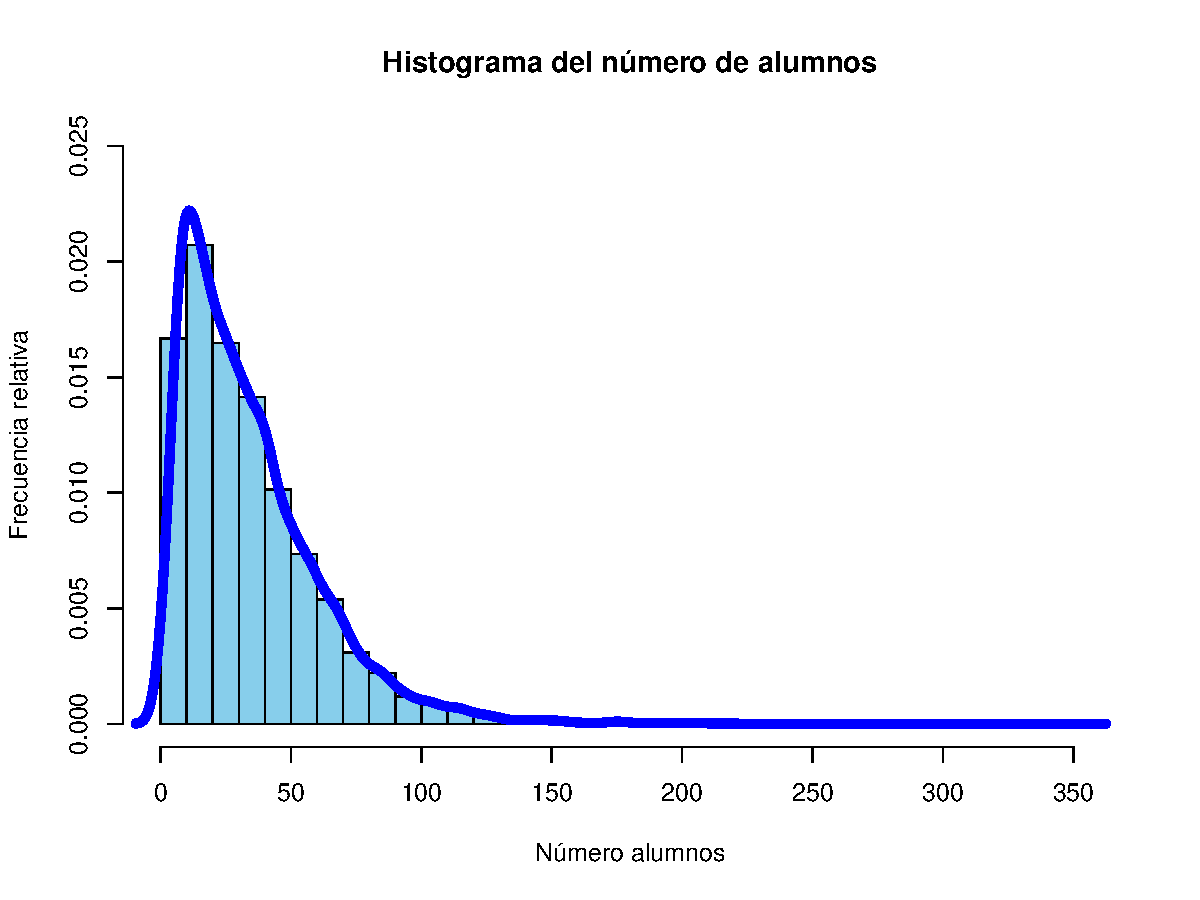
\includegraphics[scale = 0.8]{histograma_FR_num_alum_x_gpo_x_sem.pdf} %width=\textwidth
\caption{\textit{Densidad ajustada del tamaño de grupo}}\label{densidad_tamGpo}
\end{figure}

Con la función \verb@fitdist(vec_alumnos, distr = "pois")@, en R, le ajustamos una distribución Poisson a los datos. Nos arrojó el valor estimado de $\lambda$. El resumen del modelo lo podemos ver en la figura \ref{fitdistPois_tamGpo}.

\begin{figure}[H]
\centering
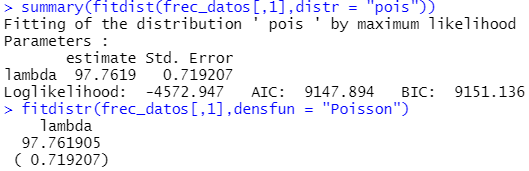
\includegraphics[scale = 1]{fitdist_poisson_tam_gpo} %width=\textwidth
\caption{\textit{Resumen del modelo ajustado para el tamaño de grupo}}\label{fitdistPois_tamGpo}
\end{figure}
